\chapter{Análisis de atenuación e intensidades}
\label{cap:cal_intensidad}

Una tomografía permite realizar dos tipos de mediciones cuantitativas, principalmente. 
En primer lugar, mediciones geométricas (longitudes, áreas, volúmenes, etc.), cuya precisión
depende de la alineación y calibración geométrica realizada al equipo, como se explicó en
el capítulo anterior. Por otro lado, se pueden realizar mediciones del coeficiente de
atenuación lineal en cada voxel del objeto. Este valor depende enteramente de la
intensidad del haz que llega a cada pixel del detector y de los cálculos realizados por el
algoritmo de reconstrucción. Este último, al igual que para con las características geométricas,
asume una serie de condiciones del haz incidente que, de no cumplirse, alterarían las mediciones
de $\mu(x,y,z)$ respecto del valor real. Por lo tanto, es necesario realizar una ``calibración de
intensidad'' del haz, por medio de correcciones a las proyecciones obtenidas en la adquisición.
En este capítulo, se presentan algunos métodos de procesamiento de imágenes, previo a la
reconstrucción.

\section{Métodos experimentales}

Todos los algoritmos de reconstrucción, en general, asumen que el haz que llega al detector
cuando no hay un objeto al medio tiene una intensidad uniforme a lo largo de toda la pantalla, y
que se mantiene constante en el tiempo \cite{Als-Nielsen2011}. Sin embargo, debido a la naturaleza de la fuente ambas
cosas no se cumplen. Por un lado, el haz no es uniforme en toda el área proyectada, puesto que
su intensidad disminuye suavemente a medida que se aleja del centro del círculo proyectado. Además,
como se observa en los gráficos de la figura \ref{fig:intensidad}, esta disminución tampoco tiene
una simetría en particular. 

Por otro lado, la intensidad que llega a cada pixel del detector tampoco es la misma en el tiempo.
Esta depende de cuánto tiempo haya pasado desde que se encendió la fuente, la estabilidad de los
X, la electrónica del detector, entre otros factores. En la figura
\ref{fig:intensidad_tiempo}, se observa cómo cambia la intensidad promedio en un ROI del fondo,
en función del número de imagen radiográfica (relacionado al tiempo transcurrido, según el tiempo
de adquisición de cada imagen) en un conjunto adquirido para una tomografía. Así, se
puede ver un máximo inicial (correspondiente a la fuente recién encendida), al que le sigue una
rápida disminución hasta un mínimo, y una eventual estabilidad alrededor de un valor entre ambos
extremos.

También es importante destacar que, debido al diseño del detector, todas las imágenes radiográficas
adquiridas presentan un patrón hexagonal cuya forma es constante en todo el fondo, y cuyos hexágonos
tienen un tamaño aproximado de 25 pixeles. Este patrón aparece debido a una grilla hexagonal
incorporada en la pantalla del detector (como una protección que viene de fábrica), y es de
interés eliminar su presencia en las imágenes.

\begin{figure}[htpb]
    \centering
    \begin{subfigure}{0.49\textwidth}
        \begin{overpic}[width=\linewidth]{images/intensidad_a.png}
            \put(3, 69){\colorbox{black!60}{\color{white}\bfseries\large (a)}}
        \end{overpic}
    \end{subfigure}
    \hfill
    \begin{subfigure}{0.49\textwidth}
        \begin{overpic}[width=\linewidth]{images/intensidad_b.png}
            \put(3, 69){\colorbox{black!60}{\color{white}\bfseries\large (b)}}
        \end{overpic}
    \end{subfigure}
    \caption{\textbf{a)} Intensidad del haz de rayos X en toda la sección cónica sobre el detector,
    visualizada a través de un mapa de colores (esta es una de las imágenes utilizadas en la alineación
    fuente-detector, ver fig. \ref{fig:res_alin_fuente}). La intensidad no es uniforme en toda el área.
    \textbf{b)} Intensidad del haz de rayos X que llega al detector en su posición final, en función de
    la posición de cada pixel. Como se observa, el centro tiene mayor intensidad, y uno de sus lados
    tiene una mayor disminución (hasta un 50\% del valor máximo).}
    \label{fig:intensidad}    
\end{figure}

\begin{figure}[htpb]
    \centering
    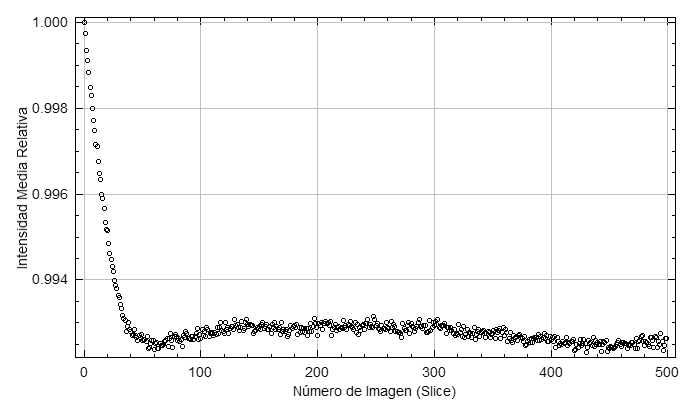
\includegraphics[width=0.8\textwidth]{images/intensidad_tiempo.png}
    \caption{Intensidad media relativa del haz de rayos X que llega al detector (a un ROI
    arbitrario de aproximadamente 100x100 pixeles), en función del número de imagen radiográfica
    adquirida para una tomografía. Se observa un máximo inicial, seguido de una rápida
    disminución y una eventual estabilización a un valor aproximado del 99.3\% del valor inicial.}
    \label{fig:intensidad_tiempo}    
\end{figure}

Para solucionar estas diferencias de la intensidad en área y tiempo, se realizan dos tipos de correcciones
distintas, presentadas a continuación. Además, la corrección en área también se encarga de la grilla hexagonal.

\subsection{Corrección de Campo Plano (FFC - Flat Field Correction)}

El objetivo de este método es corregir la intensidad del haz en función de la posición del pixel,
para un tiempo determinado, con tal de obtener uniformidad en el área. También busca corregir
posibles irregularidades en la respuesta de cada pixel, propias del detector, y la presencia del
patrón hexagonal. Para esto, además de las proyecciones radiográficas del objeto, es necesario
adquirir dos tipos de imágenes adicionales: imágenes con solo el haz incidente (sin objeto) o
\textit{flats}, e imágenes con la fuente apagada (sin haz incidente) o \textit{darks}.
Estas imágenes se adquieren con el mismo tiempo de exposición que las proyecciones radiográficas,
así como mismo voltaje y corriente de la fuente. Al mismo tiempo, es recomendable adquirir varias
imágenes de cada tipo, para luego obtener un promedio de flats y uno de darks, con el fin de reducir
el ruido.

Una vez adquiridas estas imágenes, se realiza la corrección de la intensidad $I(x,y)$ de cada pixel,
en cada proyección radiográfica, a través de la siguiente fórmula:

\begin{equation}
    I_{FFC}(x,y) = \dfrac{I(x,y) - I_{dark}(x,y)}{I_{flat}(x,y) - I_{dark}(x,y)} \times C
    \label{eq:FFC}
\end{equation}
donde $I_{dark}(x,y)$ y $I_{flat}(x,y)$ son los valores del pixel $(x,y)$ en las imágenes promedio
de darks y flats respectivamente, y $C$ es una constante de normalización que se puede elegir
arbitrariamente. En este trabajo, se definió $C$ como la moda de la intensidad (es decir, el valor
más repetido) en la imagen promedio de todas imágenes \textit{flats}. De esta forma,
se mantiene la escala de intensidad a un valor similar al que se tenía antes de la corrección.
Es importante destacar que todos los cálculos que se realizan a partir de la fórmula \ref{eq:FFC}
deben hacerse con imágenes en 32-bit, ya que en la mayoría de los casos, los valores de $I - I_{dark}$
y $I_{flat} - I_{dark}$ son muy similares, y la división entre ambos en 8 o 16 bits puede generar
errores de redondeo a 1, perdiendo la información que se busca (esto no implica que las imágenes deban
ser adquiridas en 32-bit, solamente es necesario en el cálculo).

$I_{flat}(x,y)$ contiene toda la información sobre la distribución de intensidad del haz, así como
la presencia del patrón hexagonal. Por otro lado, $I_{dark}(x,y)$ contiene información sobre el
ruido de fondo del detector, que se resta para eliminar su influencia en la corrección. De esta forma,
la fórmula \ref{eq:FFC} corrige la intensidad de cada pixel, obteniendo un haz incidente uniforme
en toda el área. 

Esta corrección es también una opción de configuración en el software del detector. Sin embargo, se encontraron dificultades
a la hora de cargar las imágenes de flats y darks en el software, por lo que para tener un mayor
control sobre el proceso, se decidió implementar la corrección de forma manual, a trevés de un
macro en FIJI (ver Apéndice B.6).

\subsection{Corrección de uniformidad temporal}

El objetivo de este método es corregir la intensidad del haz en función del tiempo (efectivamente,
número de imagen radiográfica), para obtener uniformidad temporal. Para esto, se trabaja directamente
sobre las proyecciones radiográficas, sin necesidad de aquirir imágenes adicionales.
Se considera que la intensidad relativa del haz en cada pixel, cambia aproximadamente de la misma
forma a lo largo del tiempo (es independiente de la posición del pixel). De esta forma, se corrige
cada imagen a partir de la siguiente fórmula:

\begin{equation}
    I_{T}(n,x,y) = \dfrac{I(n,x,y)}{I_{ROI}(n)} \times I_{ROI}(n_f)
    \label{eq:corr_temporal}
\end{equation}
donde $I(n,x,y)$ es la intensidad del pixel $(x,y)$ en la imagen radiográfica número $n$, $I_{ROI}(n)$
es la intensidad media en un ROI del fondo para la imagen número $n$, y $I_{ROI}(n_f)$ es la intensidad
media en el mismo ROI para la última imagen radiográfica adquirida (en la que se supone que el haz ya
se estabilizó). De esta forma, se corrige cada imagen radiográfica por su intensidad relativa,
obteniendo una serie de imágenes con una haz uniforme a lo largo del tiempo. El ROI seleccionado
debe contener solamente pixeles del fondo (sin presencia de ningún objeto), y en principio el tamaño
no es relevante, siempre y cuando se haya realizado la corrección FFC previamente a todo el set, y
esta sea satisfactoria.
Para implementar este método, se realizó un macro en FIJI (ver Apéndice B.7).

\section{Resultados} 

Se diseñaron los macros en FIJI para realizar ambas correcciones, y se aplicaron con distintos objetos
para evaluar su efectividad. En este caso, se utilizó una vértebra para adquirir proyecciones
radiográficas. Se tomaron 500 imágenes en distintas posiciones angulares (cada 0.72$^{\circ}$),
y se tomaron 5 imágenes de flats y 5 de darks para obtener los promedios. La vértebra se encuentra
en uno de los porta-muestras cilíndricos, suspendida en algodón.

En primer lugar se realizó la corrección FFC como se describió antes. Para verificar la efectividad
de esta, también se realizó sobre el conjunto de imágenes \textit{flats}. En la figura \ref{fig:res_FFC}
se observa la imagen promedio de los \textit{flats} y uno arbitrario corregido, con un mapa de color
en intensidad. En la figura \ref{fig:histogramas} se observan los histogramas de cada una de las
imágenes. Para un análisis más en detalle, se midió la intensidad media, desviación estándar y
relación señal-ruido en 154 ROIs cuadrados de 100 px de lado, distribuidos de forma equiespaciada
en toda la imagen. En la tabla \ref{tabl:FFC_flat} se encuentran los resultados. En las figuras
\ref{fig:vertebra}.a y \ref{fig:vertebra}.b se muestra una proyección arbitraria de la vértebra
y su corrección por FFC.

Por otro lado, se aplicó una transformada de Fourier rápida (FFT) al promedio de flats y a uno
de los corregidos, con el fin de estudiar la presencia de estructuras periódicas o patrones
antes y después de la corrección. Los espectros obtenidos se encuentran en la figura
\ref{fig:espectros_fourier}. Las figura \ref{fig:vertebra}.c y \ref{fig:vertebra}.d son las transformadas de Fourier
de una de una radiografías de la vertebra y su versión corregida.

\begin{figure}[htpb]
    \centering
    \begin{subfigure}{0.49\textwidth}
        \begin{overpic}[width=\linewidth]{images/Flat_Avg.png}
            \put(3, 69){\colorbox{black!60}{\color{white}\bfseries\large (a)}}
        \end{overpic}
    \end{subfigure}
    \hfill
    \begin{subfigure}{0.49\textwidth}
        \begin{overpic}[width=\linewidth]{images/flat_ffc.png}
            \put(3, 69){\colorbox{black!60}{\color{white}\bfseries\large (b)}}
        \end{overpic}
    \end{subfigure}
    \caption{Mapas de intensidad (16 bit) en el promedio de 5 imágenes \textit{flat} (\textbf{a)})
    y en uno de estos flats corregidos por \textit{flat field correcction} (\textbf{b)}).}
    \label{fig:res_FFC}    
\end{figure}

\begin{figure}[htpb]
    \centering
    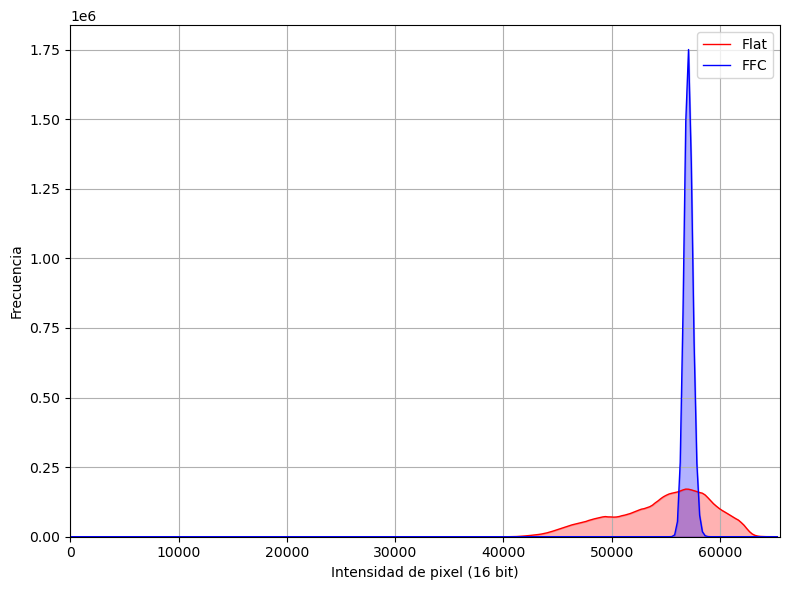
\includegraphics[width=0.55\textwidth]{images/histogramas.png}
    \caption{Histogramas correspondientes al promedio de 5 \textit{flats} (rojo), y a uno de estos
    corregido por \textit{Flat Field Correction} (azul) y normalizado con la moda de las
    intensidades del promedio de \textit{flats}.}
    \label{fig:histogramas}
\end{figure}

\begin{figure}[htpb]
    \centering
    \begin{subfigure}{0.45\textwidth}
        \begin{overpic}[width=\linewidth]{images/FFT_Flat_Avg.png}
            \put(3, 90){\colorbox{black!60}{\color{white}\bfseries\large (a)}}
        \end{overpic}
    \end{subfigure}
    \hfill
    \begin{subfigure}{0.45\textwidth}
        \begin{overpic}[width=\linewidth]{images/FFT_flat_ffc.png}
            \put(3, 90){\colorbox{black!60}{\color{white}\bfseries\large (b)}}
        \end{overpic}
    \end{subfigure}
    \caption{Espectros de Fourier del promedio de 5 imágenes \textit{flat} (\textbf{a}) y de
    uno de estos flats corregidos por \textit{flat field correction} (\textbf{b}).}
    \label{fig:espectros_fourier}    
\end{figure}

\begin{table}[htpb]
    \centering
    \caption{Promedio de parámetros estadísticos en 154 ROIs.}
    \begin{tabular}{|c|c|c|c|}
        \hline
        \textbf{Imagen} & \textbf{$VM$} & $\mathbf{\sigma}$ & \textbf{SNR} \\
        \hline
        Promedio de flats & $55100 \pm 300$ & $881 \pm 7$ & $63.0 \pm 0.5$ \\
        Flat-FFC & $57210 \pm 10$ & $367 \pm 2$ & $156.7 \pm 0.7$ \\
        \hline
    \end{tabular}
    
    \label{tabl:FFC_flat}
\end{table}

\begin{figure}[htbp]
    \centering
    % Primera fila
    \begin{overpic}[width=0.49\linewidth]{images/vertebra.png}
        \put(2, 70){\colorbox{black!50}{\color{white}\bfseries\large (a)}}
    \end{overpic}\hfill
    \begin{overpic}[width=0.49\linewidth]{images/vertebra_ffc.png}
        \put(2, 70){\colorbox{black!50}{\color{white}\bfseries\large (b)}}
    \end{overpic}
    
    \vspace{2ex} % Espaciado entre filas
    
    % Segunda fila
    \begin{overpic}[width=0.49\linewidth]{images/vertebra_fft.png}
        \put(2, 90){\colorbox{black!50}{\color{white}\bfseries\large (c)}}
    \end{overpic}\hfill
    \begin{overpic}[width=0.49\linewidth]{images/vertebra_ffc_fft.png}
        \put(2, 90){\colorbox{black!50}{\color{white}\bfseries\large (d)}}
    \end{overpic}
    
    \caption{\textbf{a)} Proyección radiográfica de una vértebra, con mapa de color de intensidad.
    \textbf{b)} Proyección radiográfica de una vértebra, corregida por \textit{flat field correction}.
    \textbf{c)} Espectro de Fourier (por FFT) de la proyección de la vértebra sin corregir (a).
    \textbf{d)} Espectro de Fourier (por FFT) de la proyección de la vértebra, corregida por
    \textit{flat field correction} (b).}
    \label{fig:vertebra}
\end{figure}

Por último, se aplicó la corrección de uniformidad temporal a las 500 imágenes corregidas por FFC,
y se observó la intensidad media en el mismo ROI del fondo para cada imagen, antes y después
de la corrección. Los resultados se encuentran en la figura \ref{fig:res_corr_temporal}.

\begin{figure}[htpb]
    \centering
    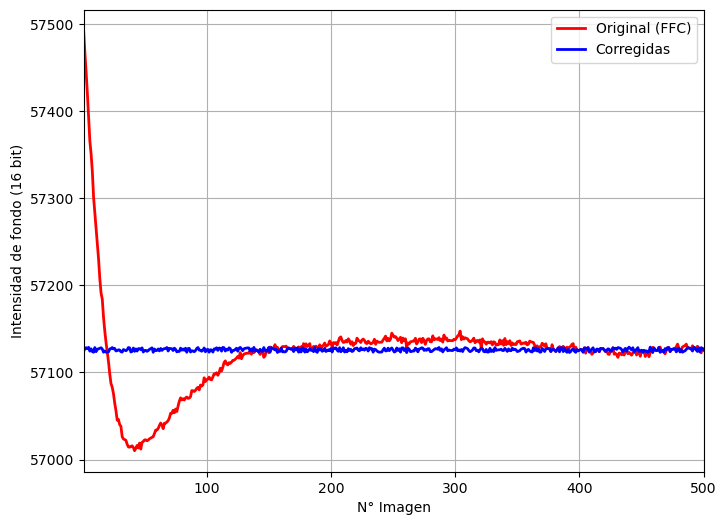
\includegraphics[width=0.8\textwidth]{images/corr_temp.png}
    \caption{Intensidad media relativa del haz de rayos X que llega al detector (a un ROI
    arbitrario del fondo), en función del número de imagen radiográfica
    adquirida para una tomografía, antes (rojo) y después (azul) de la corrección de uniformidad
    temporal.}
    \label{fig:res_corr_temporal}    
\end{figure}

\section{Discusiones}

Observando la figura \ref{fig:res_FFC}, se puede ver que la corrección FFC logra uniformizar efectivamente
la intensidad del haz en toda el área detectada. Esto mismo se puede ver en el histograma de la figura
\ref{fig:histogramas}, donde se pasa de tener un rango de intensidades de fondo entre aproximadamente
40000 y 70000 (más de 20000 niveles de intensidad), a uno mucho más reducido de entre 56000 y 58000
(menos de 2000 niveles). También la forma del histograma cambia tras la corrección, pasando de una distribución
asimétrica con dos picos distintivos (que podrían sugerir la presencia de dos ``características'' distintas,
el fondo real por un lado y el patrón hexagonal por otro), a una distribución simétrica de un solo pico,
similar a una distribución normal. Esto implica que la desviación estándar es causada principalmente por
ruido blanco, y no por otros elementos (que es lo que se desea lograr).

El histograma no es suficiente para observar la distribución espacial de la intensidad. Esto se observa
en la figura \ref{fig:res_FFC}, y con valores más concretos en la tabla \ref{tabl:FFC_flat}. La idea
de la corrección FFC es reducir la variabilidad de intensidad en cada parte del fondo, y así aumentar
la relación señal-ruido en todas las regiones por igual. Se puede ver en la tabla que esto efectivamente
sucede al aplicar la corrección. A través de esta, se logra reducir la desviación estándar, en cada ROI de
100x100 pixeles, en un factor de aproximadamente 2.4, aumentando de la misma manera el $SNR$ del fondo.
Una disminución de la desviación estándar también implica un aumento de la relación contraste-ruido, lo
que permite distinguir mejor distintas fases en una muestra. También en la figura \ref{fig:vertebra} se
observa el cambio que produce la corrección, cn mayor claridad al ver el fondo.

También a simple vista se puede notar la desaparición del patrón hexagonal en el fondo corregido.
Esto se puede observar de forma más clara y general en los espectros de Fourier de la figura
\ref{fig:espectros_fourier}. En la imagen original, se presentan una serie de picos de alta intensidad,
distribuidos en una red de Bravais triangular, correspondiente a la recíproca de una red hexagonal.
Estos picos se corresponden con los pixeles más oscuros distribuidos en una grilla hexagonal. Después
de la corrección, ningungo de estos picos permanece, lo que suguiere la desaparición por completo
de la grilla. Por otro lado, en el primer espectro de Fourier también se observan dos líneas rectas de
mayor intensidad (una vertical y otra horizontal). Estos se corresponden en primer lugar, al hecho
que la transformada de Fourier (que se define sobre un espacio infinito) se aplica al espacio finito
que es la imagen. Pero también se debe a la presencia de estructuras de filas y columnas de pixeles
con intensidades similares, propias del sistema electrónico del detector (estas son algo visibles
en la imagen de la figura \ref{fig:res_FFC}.a). Al restar la imagen \textit{Dark} durante la corrección,
estas estructuras desaparacen, lo que en el espectro de Fourier se observa como una disminución
drástica de estas dos líneas rectas.

En una radiografía de una muestra típica (un hueso por ejemplo), no suele haber componenetes de alta
frecuencia, esto es, no suele haber muchos cambios de fase en una sección muy pequeña (del orden de un
pixel), por lo que las componentes propias de la muestra se encuentran contenidas en el centro de 
de la imagen de la transformada, la cual no es afectada por estos cambios. Esto se observa con
mayor claridad al estudiar la figura \ref{fig:vertebra}. A pesar de que la imagen de la vértebra
sea mucho más ``compleja'' que un fondo blanco como el de la figura \ref{fig:res_FFC}, sus espectros
de Fourier no son muy distintos, ya que los picos más intensos se encuentran en el centro de la imagen
(frecuencias bajas), mientras que el patrón hexagonal y las líneas horizontales y verticales se distinguen
fácilmente del resto. Al aplicar la corrección FFC, son estos últimos componentes los que desaparecen
o se atenúan drásticamente, mientras que el efecto en el centro es menor.

Finalmente, se observa la efectividad de la corrección temporal de la intensidad en la figura
\ref{fig:res_corr_temporal}. El resultado es una intensidad constante, más un ruido blanco
propio del sistema. De esta forma, las proyecciones presentan uniformidad del fondo en área
y tiempo, permitiendo una reconstrucción más fiel de los valores de gris de voxel. Además,
estos resultados son fundamentales para poder realizar mediciones reales a partir de los
niveles de grises, como el coeficiente de atenuación o la densidad en un mismo material, ya
que permiten obtener valores consistentes para distintas tomografías (siempre y cuando los
parámetros de voltaje y corriente de la fuente sean los mismos). Este es un paso esencial
para poder determinar una calibración del nivel de gris en una tomografía.